% This is part of Un soupçon de mathématique sans être agressif pour autant
% Copyright (c) 2015
%   Laurent Claessens
% See the file fdl-1.3.txt for copying conditions.

%--------------------------------------------------------------------------------------------------------------------------- 
\subsection*{Patron d'un cône}
%---------------------------------------------------------------------------------------------------------------------------

Ceci est un petit cône en papier :
\begin{center}
    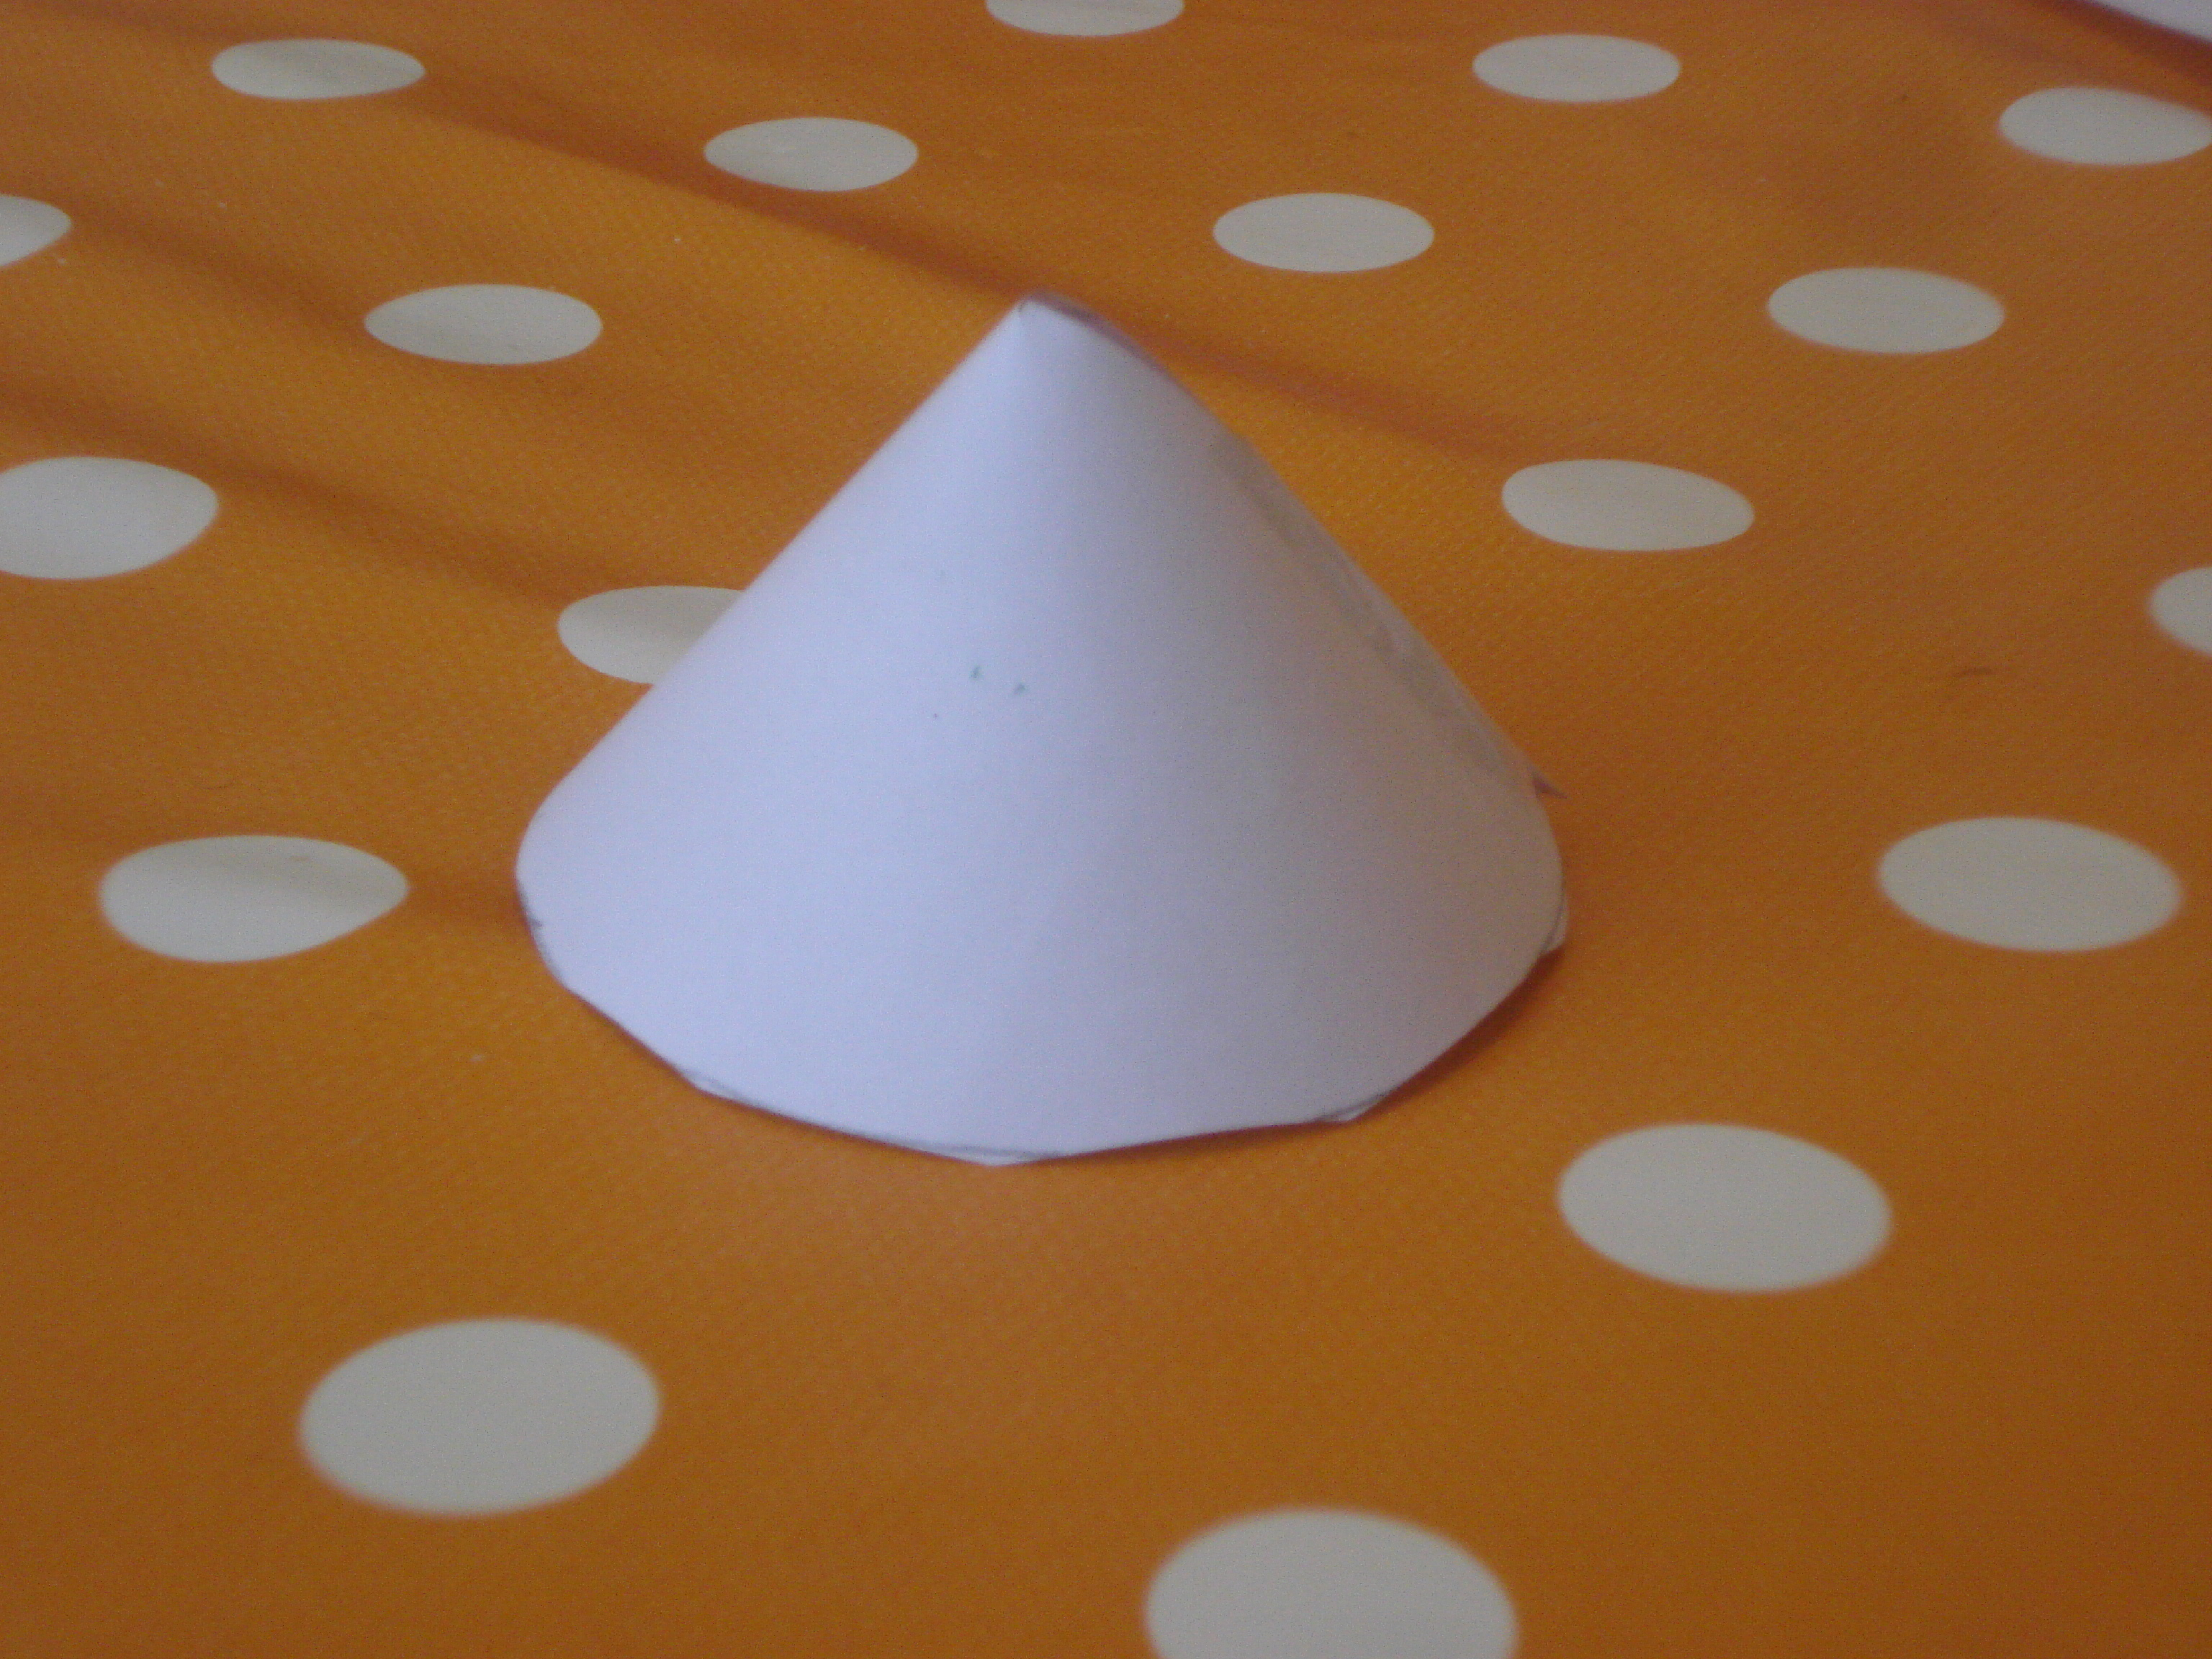
\includegraphics[width=5cm]{cone_papier.pdf}
\end{center}

\begin{enumerate}
    \item
        Comment réalise-t-on ce pliage ? Le faire.
    \item
        Comment découper le papier pour obtenir au bout du compte un cône dont le rayon de la base soit \SI{3}{\centi\meter} et la hauteur \SI{4}{\centi\meter} ?
\end{enumerate}
